\documentclass[../main.tex]{subfiles}
\begin{document}
\newpage
\section{Appendix}

\begin{figure}[H]
\centering
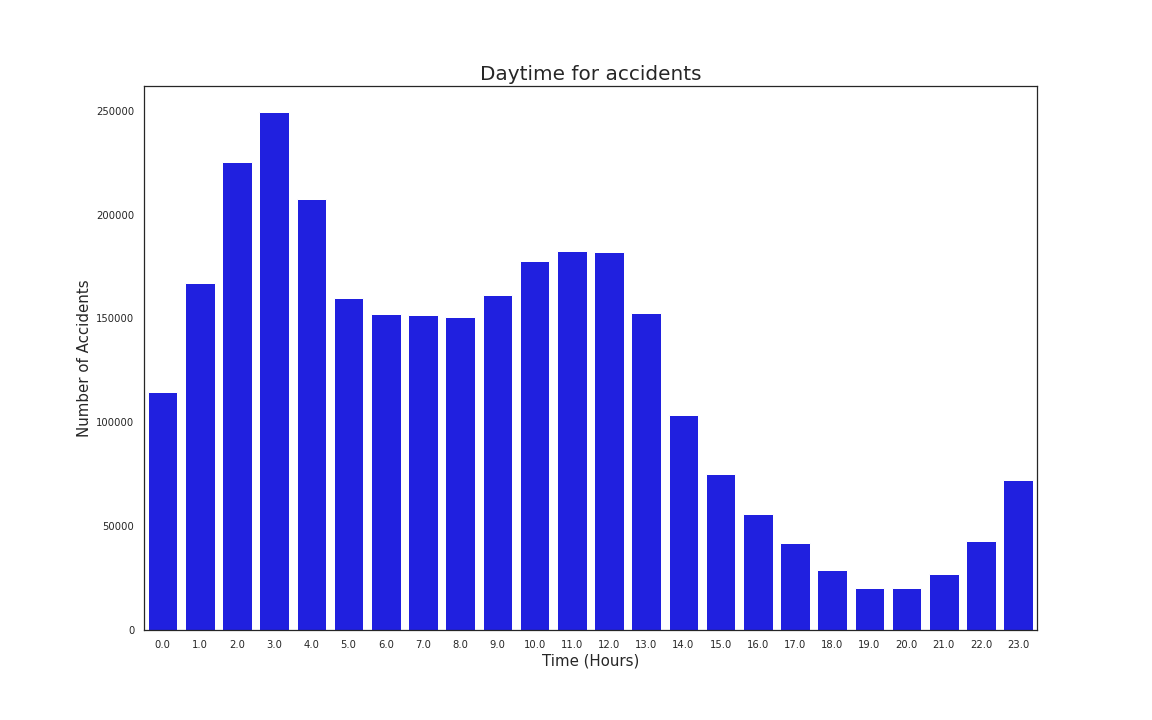
\includegraphics[width=15cm]{Images/accident_hours.png}
\caption{Which hour during the day that accidents occur.}
\label{fig:accident_hour}
\end{figure}

\begin{figure}[H]
\centering
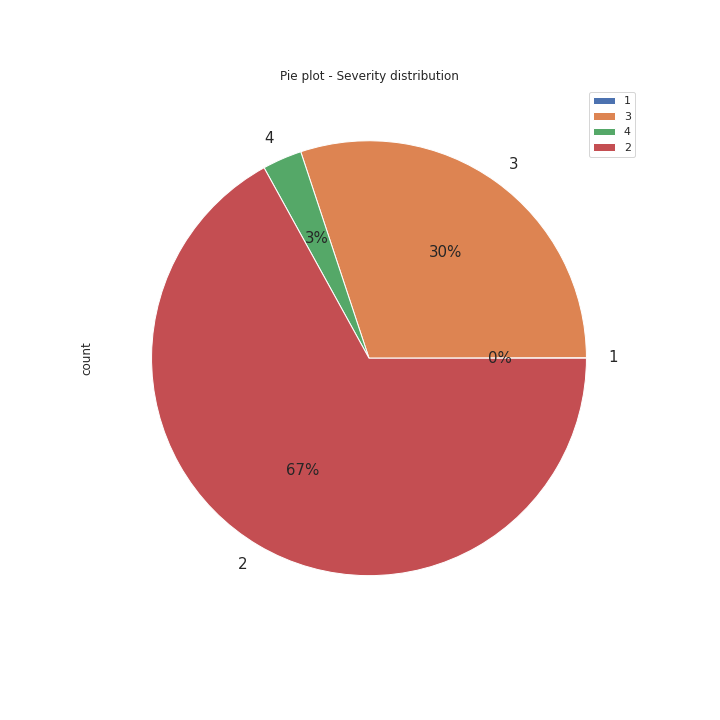
\includegraphics[width=15cm]{Images/pie_severity_dist.png}
\caption{Distribution of severity.}
\label{fig:pie_severity}
\end{figure}

\begin{figure}[H]
\centering
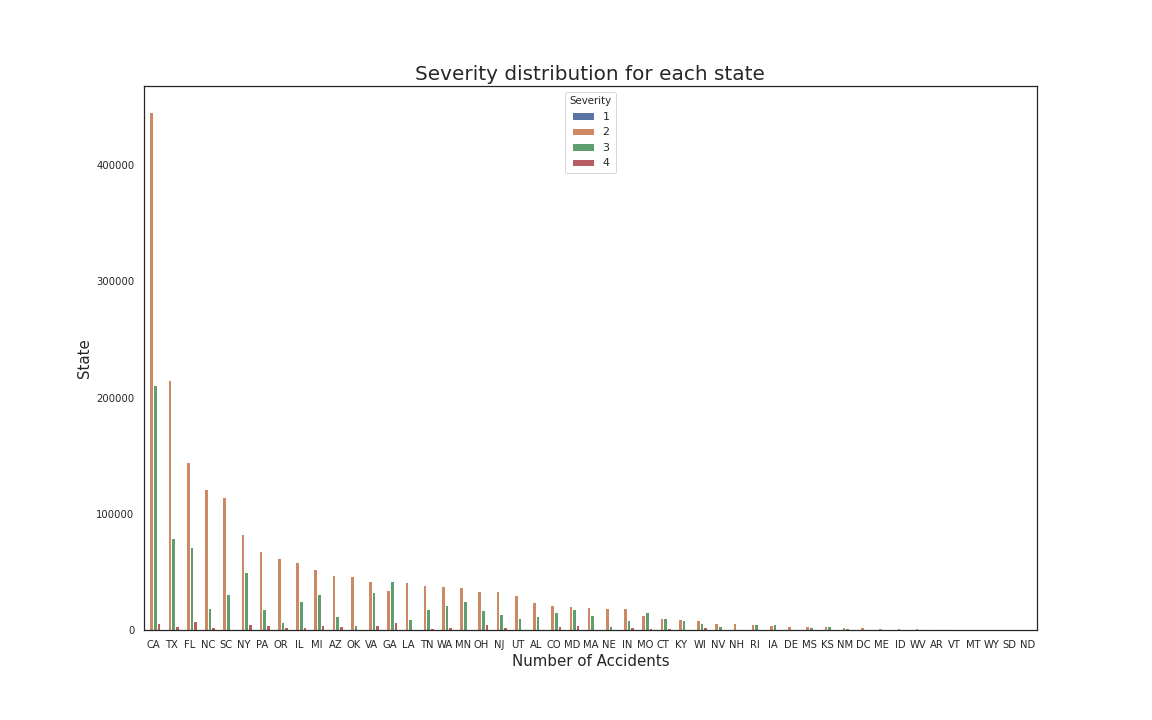
\includegraphics[width=15cm]{Images/severity_dist_class_state.png}
\caption{Distribution on severity in each state.}
\label{fig:severity_dist_class}
\end{figure}

\begin{figure}[H]
\centering
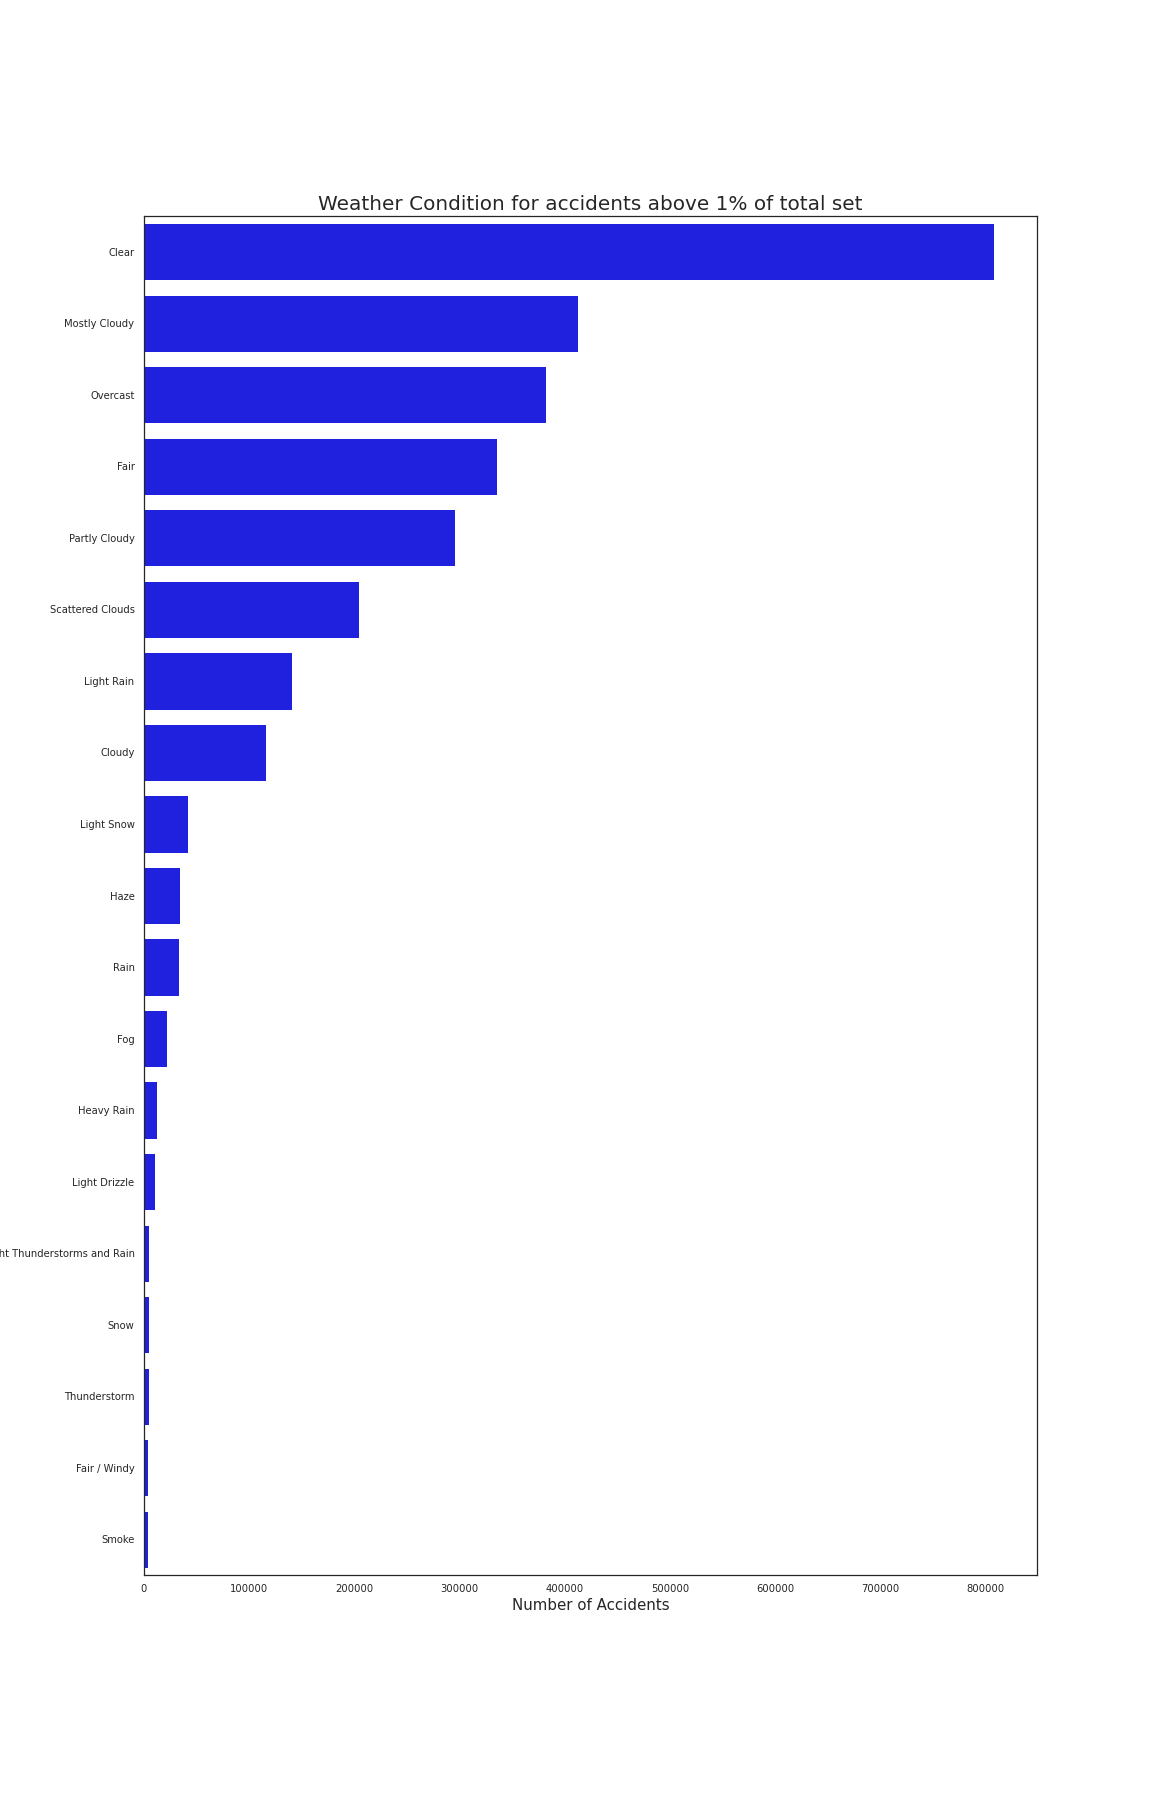
\includegraphics[width=15cm]{Images/weather_cond_dist.png}
\caption{Top weather conditions for accidents.}
\label{fig:weather_cond_dist}
\end{figure}

\begin{figure}[H]
\centering
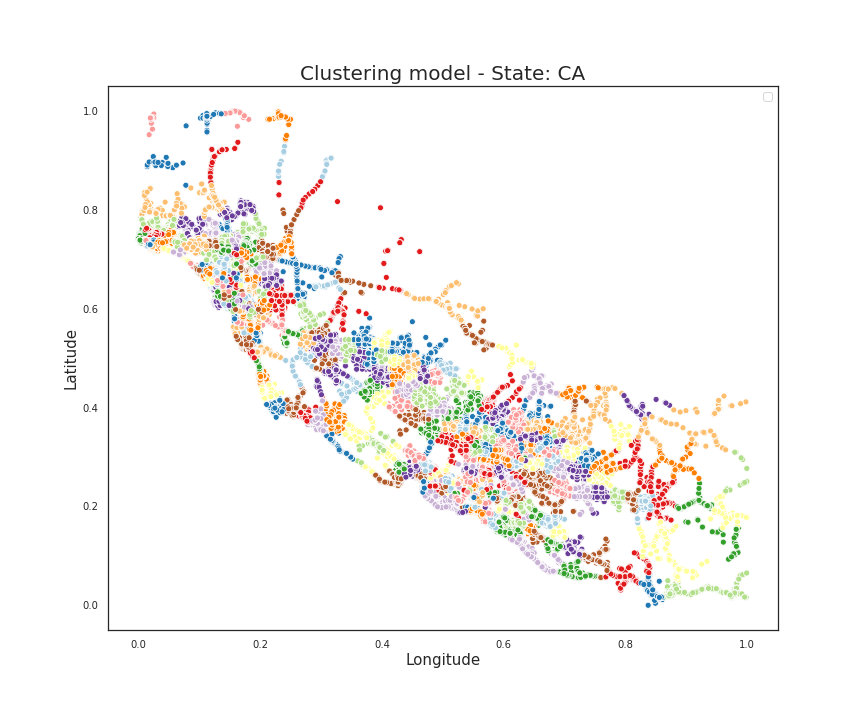
\includegraphics[width=15cm]{Images/Clustering_centroids.png}
\caption{Distribution of centroids for the state CA, gives an overview of what the centroids are covering.}
\label{fig:Clustering_centroids}
\end{figure}

\end{document}

